\chapter{Dispersed phase simulation in BIMER}
	\label{ch9:BIMER_lagrangian}

\section{Introduction}

The previous chapter has reported the resolved atomization simulations performed through one multipoint injector of the BIMER configuration. The lagrangian injector learning process was applied to get a in-plane, spatially distributed spray. This spray conforms a lagrangian injector that is used in this chapter to initialize the liquid phase dispersed-phase simulations. The dense core was also characterized: these information can be used in this chapter to impose an actuator with the ALM method that perturbs the gaseous phase similarly to a jet dense column. Due to rotational symmetry in the multipoint stage, the obtained SLI and actuator can be extrapolated to the remaining multipoint holes to perform liquid injection and gaseous phase perturbation in the full configuration. This chapter reports the results of \hl{one (two?)} dispersed-phase simulation\hl{(s)} of BIMER with the SLI methodology.

In first place, the computational setup is explained in $\S$\ref{ch9:sec_computations_setup}. The multipoint injection is briefly detailed here, while the pilot injection performed with the LISA injection model is thoroughly explained. Then, available experimental results for this configuration and the operating point chosen, which can be used for computational validation, obtained by \citeColor[renaud_high-speed_2015] are summarized in $\S$\ref{ch9:sec_expe_results_LGS_BIMER}. The SLI flowchart, which was generally detailed in Figure \ref{fig:SLI_graphic_description} for a JICF, is extended to BIMER in $\S$\ref{sec:ch9_BIMER_SLI_flowchart}. Next, the SLI used for lagrangian injector and the effect of the proposed ALM in the gaseous field are reported in $\S$\ref{sec:ch9_BIMER_BCs_for_phases}. Finally, the results from \hl{one (two)}  simulation\hl{(s)} are reported and discussed in $\S$\hl{\textbf{XX}}. \hl{It is shown that ...}





\section{Computational setup}
\label{ch9:sec_computations_setup}

For performing dispersed phase simulations, the operating point defined in Table \ref{tab:liquid_operating_point_Renaud} is simulated. The staging factor is $\alpha = 15$, meaning that $15 \%$ of the total liquid flow rate is injected through the pilot stage and the remaining liquid through the multipoint. For total flow rate of $\dot{m}_l = 1.64 g s^{-1}$, the multipoint stage injects a total $\dot{m}_{l,takeoff} = 1.39 g s^{-1}$ (hence $0.139 g s^{-1}$ per injector), and a value of $\dot{m}_{l,pilot} = 0.25 g s^{-1}$ is introduced through the pilot stage.

\begin{table}[!h]
\centering
\caption{Operating point to perform gaseous and two-phase simulations tested by \citeColor[renaud_high-speed_2015]}
\begin{tabular}{|c|c|c|c|}
\hline
\multicolumn{4}{|c|}{\textbf{Air properties}} \\
\hline
$\dot{m}_g$ [g s$^{-1}$] & $T_g$ [K] & $\rho_g$ [kg m$^{-3}$]  & $\mu_g$ [Pa s]  \\
\hline
43.1 & 433 & 0.816382 & $2.3911 \cdot 10^{-5}$ \\
\hline
\hline
\multicolumn{4}{|c|}{\textbf{Liquid properties}} \\
\hline
$\dot{m}_l$ [g s$^{-1}$] & $\rho_l$ [kg m$^{-3}]$   & $\mu_l$ [Pa s]   & $\sigma$ [N m$^{-1}$]   \\
\hline
1.64 & 750 & $1.36 \cdot 10^{-3}$ & $25.35 \cdot 10^{-3}$ \\
\hline
\hline
\multicolumn{4}{|c|}{\textbf{Burner staging}} \\
\hline
$\alpha$ [$\%$] & $\dot{m}_{l,pilot}$ & $\dot{m}_{l,takeoff}$ & \\
\hline
15 & 0.25 & 1.39 & \\
\hline
\end{tabular}
\label{tab:liquid_operating_point_Renaud}
\end{table}


\subsection{Multipoint stage injection}

For the multipoint stage, the injectors obtained in Chapter \ref{ch:bimer_resolved_atomization} ($\S$ \textbf{Section??}) are used. These injectors were, however, obtained from the simulations of one single injector. In order to initialise the rest of multipoint injection holes (for a total of 10 in BIMER, see Figure \textbf{Figure??}), new numerical injectors need to be defined in each hole by making a revolution of the available ones. This revolution is possible due to the radial of BIMER in terms of injectors location (which are equally spaced to a distance of 25 mm from the center with a radial difference of 36 $\degree$) and the multipoint vane locations: each injection hole is located at the same location between two vanes, hence seeing the same incoming air (see Figure \textbf{Figure??})).

Each injector will deliver a mass flow rate of $\dot{m}_{l,takeoff} = 0.139 g s^{-1}$, equivalent to a flow rate of $Q_l = 185.3 mm^3 s^{-1}$.


\subsection{Pilot stage injection}

Since pilot stage has not been simulated with the injection models developed in this thesis, another methodology must be employed. Given that the pilot of BIMER injects fuel following a hollow cone configuration, the LISA model will be used \citepColor[guedot_developpement_2015]. 

The input parameters for the LISA model to inject a hollow cone spray are summarized in Table \ref{tab:LISA_model_parameters}. They intend to replicate the pilot injection by \citeColor[renaud_high-speed_2015]. For the angle, an initial value of 30 $\degree$ is chosen (Stefano first guess), it can be iterated as we keep on refining the simulations. For the rayon, I have no idea what to do.

For the injection diameter, the following correlation used by Lefebvre for pressure-swirl sprays is used:

\begin{equation}
SMD = 2.25 \left( \sigma \dot{m}_f \mu_l \right)^{0.25} \rho_g^{-0.25}  \Delta P^{-0.5}
\end{equation}

where $\Delta P$ is the pressure drop in the pilot nozzle. According to \citeColor[renaud_high-speed_2015], (p. 24, or 46 PDF), pilot liquid is injected at $2.7 MPa$ to the chamber at atmospheric pressure. By taking this pressure drop, and using the values given in Table \ref{tab:liquid_operating_point_Renaud}, this correlation provides a SMD of $15 \mu m$ (\textbf{CHECK THIS}).

\subsubsection*{LISA model for injection}

For performing pilot injection, the LISA model available in YALES2 is used \citepColor[guedot_developpement_2015]. 

\begin{equation}
X = \frac{A_a}{A_0} = \left( \frac{R_a}{R_0} \right)^2 \frac{\sin^2 \gamma_s}{1 + \cos^2 \gamma_s}
\end{equation}

where $R_a$ is the minimum injection radius, $R_0$ the maximum, and $\gamma_s$ is the mean injection angle. The inputs to the model are $\gamma_s$ and $R_0$, so from the previous equation $X$ can be obtained and the radius $R_a$ can be solved:

\begin{equation}
R_a^2 = R_0^2 X
\end{equation}

The axial velocity imposed to the particles $u_x$ is obtained through the following expression:

\begin{equation}
u_x = \frac{\dot{m}}{\rho_l \pi \left( R_0^2 - R_a^2 \right)} = \frac{\dot{m}}{\rho_l \pi R_0^2 \left( 1 - X^2 \right)} 
\end{equation}

\textbf{OJO}: in Renaud's application case ($\dot{m} = 0.25 ~ g/s$, see Table \ref{tab:LISA_model_parameters}), taking $R_0 = 0.125 ~mm$ gives an axial velocity of $u_x = 7.9 ~ m/s$. This created an almost-point injection, as it can be seen in the simulations. If we take $R_0 = 1.5 ~mm$ (the radius of the hollow cone patch), droplets are injected along all the hollow cone patch. However, the axial velocity imposed is $u_x = 0.05 ~m/s$. So we'll go towards the large radius.

\begin{table}[!h]
\centering
\caption{LISA model setup for pilot injection}
\begin{tabular}{|c|c|}
\hline
\textbf{Parameter} & \textbf{Value} \\
\hline
Mass flow rate $\dot{m} [g s^{-1}]$ & 0.25 \\
\hline
Injector radius $R_0 [mm]$ & 0.125 \\
\hline
Mean angle $\overline{\theta} [\degree]$ & 40 \\
\hline
\end{tabular}
\label{tab:LISA_model_parameters}
\end{table}

\subsection{Evaporation}

Due to the high gas ambient temperature inside the BIMER combustion chamber (433 K, see Table \ref{tab:liquid_operating_point_Renaud}), evaporation of lagrangian droplets should be considered. In this case 

\section{Experimental results from literature}
\label{ch9:sec_expe_results_LGS_BIMER}

The BIMER operating point tested in this chapter to test the SLI methodology has been chosen since it presents non-reactive experimental results that can be used for validation. These ones, shown in the PhD thesis of \citeColor[renaud_high-speed_2015], consist of the qualitative maps of SMD, axial and vertical velocities shown in Figure \ref{fig:maps_BIMER_renaud_expe_results}. Qualitative experimental results on non-reactive conditions are not available from literature, and hence a qualitative validation is not possible to this date.

\begin{figure}[h!]
\flushleft
\begin{subfigure}[b]{0.3\textwidth}
	\centering
   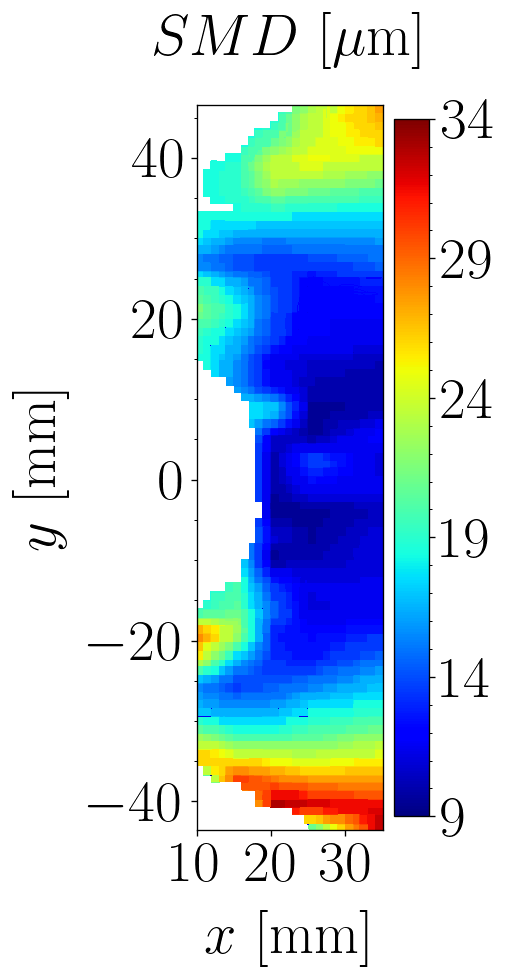
\includegraphics[scale=0.4]{./part3_applications/figures_ch9_lagrangian/expe_maps/SMD_map.png}
   %\caption{Low Weber number operating point.}
   %\label{} 
\end{subfigure}
\hspace*{0.1in}
\begin{subfigure}[b]{0.3\textwidth}
	\centering
   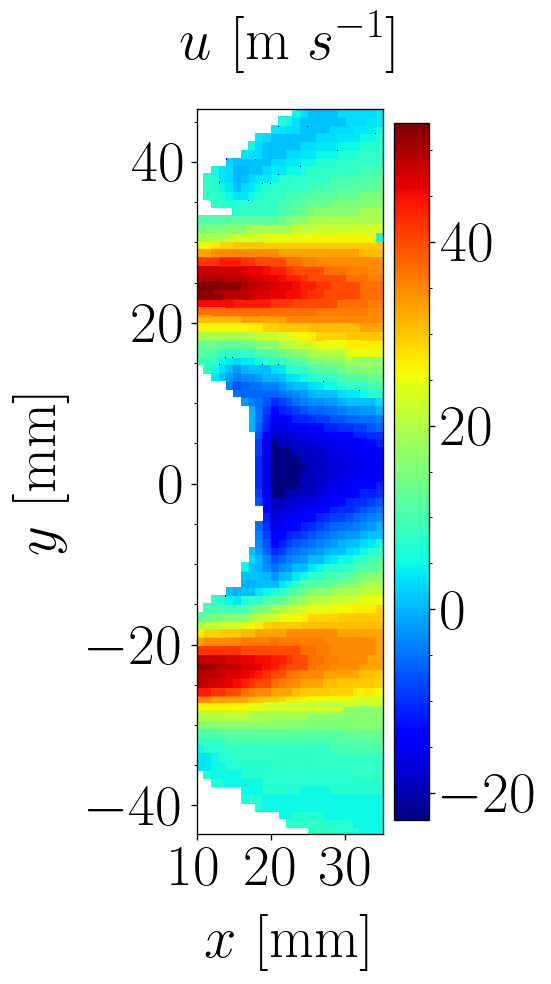
\includegraphics[scale=0.4]{./part3_applications/figures_ch9_lagrangian/expe_maps/u_axial_map.png}
   %\caption{Low Weber number operating point.}
   %\label{} 
\end{subfigure}
\hspace*{0.1in}
\begin{subfigure}[b]{0.3\textwidth}
	\centering
   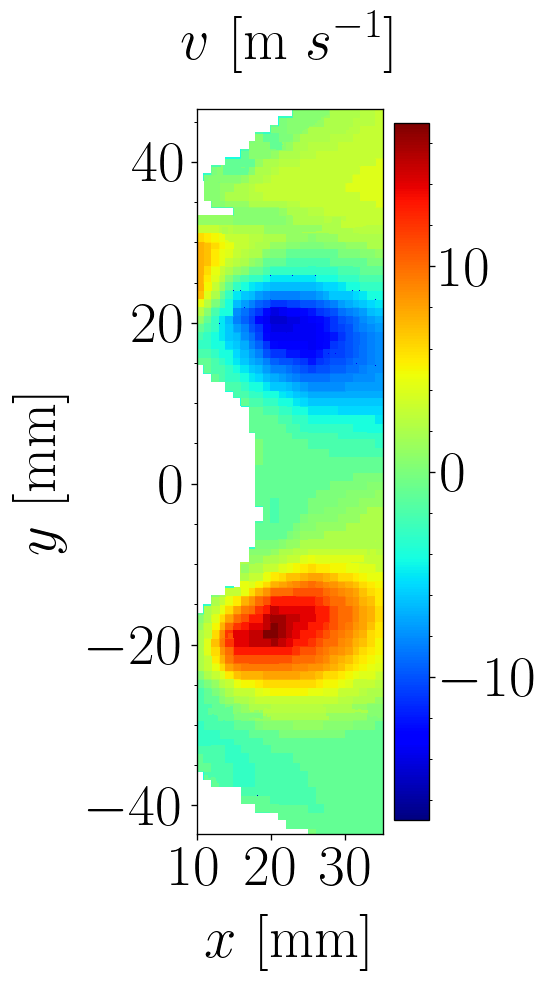
\includegraphics[scale=0.4]{./part3_applications/figures_ch9_lagrangian/expe_maps/u_vertical_map.png}
   %\caption{Low Weber number operating point.}
   %\label{} 
\end{subfigure}
\caption{Experimental maps for for $SMD$, axial velocity $u$ and vertical velocity $v$ from \citeColor[renaud_high-speed_2015].}
\label{fig:maps_BIMER_renaud_expe_results}
\end{figure}

\section{Model flowchart applied to BIMER}
\label{sec:ch9_BIMER_SLI_flowchart}

\section{Boundary condition for phases}
\label{sec:ch9_BIMER_BCs_for_phases}

\subsection{Gaseous phase}

\subsection{Liquid phase: lagrangian injector definition}

In order to initialise the liquid phase, an SLI is created from the resolved simulations of BIMER for case DX07 at the sampling plane $x/d_\mathrm{inj} = 3.33$. Following the results from the lagrangian simulations of Chapter \ref{ch6:jicf_lgs_simulations}, the injectors are obtained through convergence-driven discretization; the injection velocities are defined with a gaussian $r$ law; and the mean and RMS velocities are volume-weighted; and the secondary atomization model chosen is the Gorokhovski model with constants $K_1 = $ \hl{\textbf{XX}}, $K_2 = $ \hl{\textbf{XX}}. The resulting injectors are shown in Figure \\hl{\textbf{XX}}.


\subsection{Dispersed phase simulations}

\subsection{Effect of dense core perturbation}

\subsection{Effect of evaporation}

\section{Extrapolation of injectors to rest of multipoint holes}

The 

\subsection{Injectors geometry}

\begin{equation}
\boldsymbol{x}_0 =  \begin{pmatrix} - 38.5 ~\mathrm{mm} \\ r \cos \alpha_0 \\ r \sin \alpha_0 \end{pmatrix}
\end{equation}

\begin{equation}
\boldsymbol{x}_i =  \begin{pmatrix} - 38.5 ~\mathrm{mm} \\ r \cos \alpha_i \\ r \sin \alpha_i \end{pmatrix}
\end{equation}


\subsection{General procedure}

\begin{enumerate}

	\item Obtain parameters for SLI of injector 0 (baseline parameters):
	
	\begin{equation}
	\alpha_0  ~~ ; ~~ \boldsymbol{n}_0 ~~ ; ~~ \theta_0 = 90 - \alpha_0 - atan \left( \frac{n_y}{n_z} \right) ~~ ; 
	\end{equation}

	\item Get parameters for SLI of injector $i$ from baseline:
	
	\begin{equation}
	\alpha_i = \alpha_0 - i \Delta \alpha 
	\end{equation}
	
	\begin{equation}
	\boldsymbol{n}_i = 
	\end{equation}
	
	\begin{equation}
	\theta_1 = \theta_0
	\end{equation}
	

\end{enumerate}

\subsection{Definition of coordinate systems and operations}

The global coordinate system is:

\begin{equation}
\boldsymbol{x} =  \begin{pmatrix} x \\ y \\ z \end{pmatrix}
\end{equation}

The local (crossflow) coordinate system is:

\begin{equation}
\boldsymbol{x}^{cr} = \begin{pmatrix} x^c \\ y^c \\ z^c \end{pmatrix}
\end{equation}

with the following equivalences between local and global systems :

\begin{equation}
\boldsymbol{x}^c = \boldsymbol{n}  ~~~~ ; ~~~~ \boldsymbol{z}^c = \boldsymbol{x}  ~~~~ ; ~~~~ \boldsymbol{y}^c =  \boldsymbol{z}^c \times \boldsymbol{x}^c
\end{equation}

where the rotation matrix being:

\begin{equation}
\boldsymbol{R} = \begin{pmatrix} \boldsymbol{x}^{c^T} \\ \boldsymbol{y}^{c^T} \\ \boldsymbol{z}^{c^T} \end{pmatrix}
\end{equation}

More elegantly expresses:

\begin{equation}
\boldsymbol{R} = \begin{pmatrix} x^c_x & x^c_y & x^c_z \\ y^c_x & y^c_y & y^c_z \\ z^c_x & z^c_y & z^c_z \end{pmatrix}
\end{equation}

%\begin{equation}
%\boldsymbol{x} =  \begin{pmatrix} 1 & 2 & -3 \\ 4 & 0 & 1 \end{pmatrix}
%\end{equation}


Transformation for droplet locations is translation + rotation

\begin{equation}
\boldsymbol{x}^c_\mathrm{dr} = \boldsymbol{R} \left( \boldsymbol{x}_\mathrm{dr} -  \boldsymbol{x}_0 \right)
\end{equation}

For droplet velocities, transformation is only rotation:

\begin{equation}
\boldsymbol{u}^c_\mathrm{dr} = \boldsymbol{R} \boldsymbol{u}_\mathrm{dr}
\end{equation}

Inverse transform then:

\begin{equation}
\boldsymbol{x}_\mathrm{inj} = \boldsymbol{x}_0 + \boldsymbol{R}^{-1} \boldsymbol{x}_\mathrm{inj}^c
\end{equation}

\begin{equation}
\boldsymbol{u}_\mathrm{inj} = \boldsymbol{R}^{-1} \boldsymbol{u}_\mathrm{inj}^c
\end{equation}

\section{Towards reactive simulations}



\section{Conclusion}

In this chapter ...

Further work is required in order to accurately match the experimental results. Nevertheless, this chapter has shown the capability of SLI to initialise the spray in dispersed-phase simulations from more realistic, industrial-type multi-staged burners, and its ability to add multiphysical phenomena such as evaporation. Next steps include adding a flame kernel to ignite the reactive gas-fuel mixture and simulate combustion.